\documentclass{article}
\usepackage[utf8]{inputenc}
\usepackage{amssymb}
\usepackage{graphicx}
\usepackage{cancel}
\usepackage{chngcntr}
\setlength{\oddsidemargin}{0in}
\setlength{\textwidth}{6.5in}
\setlength{\topmargin}{-.55in}
\setlength{\textheight}{9in}
\graphicspath{{Images/}}
\counterwithin{equation}{section}


\title{Problem Set 3 (Astrophysics)}
\author{Michael Nameika}
\date{February 2022}

\begin{document}

\maketitle
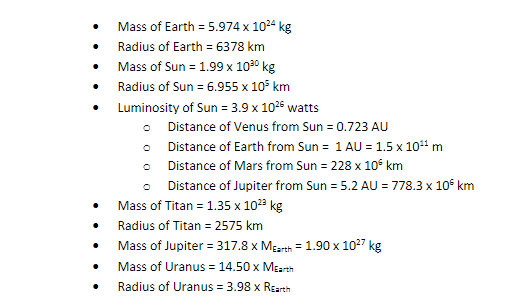
\includegraphics[scale = 0.8]{probset3data.PNG}
\section{}
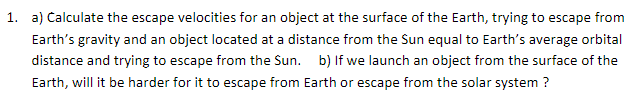
\includegraphics[scale = 0.8]{probset3num1.PNG}

Recall that the escape velocity for an object is given by 
\begin{equation}
    v_e = \sqrt{\frac{2GM}{r}}
\end{equation}
Where $M$ is the mass of the body you're trying to escape from, and $r$ is the distance from the center of mass. 
a) We wish to find the escape velocity for the Earth. Using the values for the mass and distance from the center of the Earth:
\[M_{Earth} = 5.974 \times 10^{24} \: kg\]
\[r_{Earth} = 6.378 \times 10^6 \: m\]
Plugging these values into (1.1), we will get the following:
\[v_e = \sqrt{\frac{2(6.67 \times 10^{-11} \: \cancel{kg^{-1}} \: m^{\cancel{3} \to 2} \: s^{-2})(5.974 \times 10^{24} \: \cancel{kg})}{6.378 \times 10^6 \:\cancel{m}}}\]
\[ = 11.18 \frac{km}{s}\]
so the escape velocity at the surface of the Earth is approximately $11.18 \frac{km}{s}$. Now we wish to find the escape velocity from the sun at the mean distance of the Earth from the Sun.

Using that the mass of the Sun is $M_{Sun} = 1.99 \times 10^{30} \: kg$ and the distance of the Earth from the Sun $1.5 \times 10^{11} \: m$ from the table at the beginning of the assignment, we find that the escape velocity from the Sun at Earth's distance is
\[v_e = \sqrt{\frac{2(6.67 \times 10^{-11} \: \cancel{kg^{-1}}m^{\cancel{3} \to 2}s^{-2})(1.99 \times 10^{30} \: \cancel{kg})}{1.5 \times 10^{11} \: \cancel{m}}}\]
\[ = 42068.7 \: \frac{m}{s}\]
\[ = 42.1 \frac{km}{s}\]





\section{}
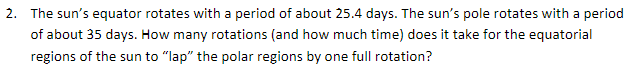
\includegraphics[scale = 0.8]{probset3num2.PNG}


We wish to find $t$ such that 
\[\frac{t}{25.4 \: days} = \frac{t}{35 \: days} + 1\]
That is, we want to find $t$ where the equator rotates one more time than the poles of the Sun. Solving, we get
\[t(\frac{1}{25.4 \: days} - \frac{1}{35 \: days}) = 1\]
\[t = \frac{1}{\frac{1}{25.4 \: days} - \frac{1}{35 \: days}}\]
\[\approx 92.6 \: days\]
Now let's find the total amount of rotations that occurred during that time:

At the equator: 
\[\Delta_{rot} = \frac{92.6 \: \cancel{days}}{25.4 \frac{\cancel{days}}{rotation}} = 3.646 \: rotations\]

At the pole: 
\[\Delta_{rot} = \frac{92.6 \: \cancel{days}}{35 \frac{\cancel{days}}{rotation}} = 2.646 \: rotations\]




\section{}
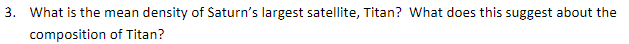
\includegraphics[scale = 0.8]{probset3num3.PNG}

From the data in the given table, we have that $M_{Titan} = 1.35 \times 10^{23} \: kg$ and $r_{Titan} = 2575 \: km$, and assuming that Titan is nearly spherical, we can calculate the average density of Titan:
\[\rho_{Titan} = \frac{1.35 \times 10^{23} \: kg}{\frac{4}{3}\pi (2.575 \times 10^6 \:m)^3}\]
\[\approx 1.888 \times 10^3 \frac{kg}{m^3}\]
\[ = 1.888 \frac{g}{m^3}\]
Thus Titan has a density roughly twice that as water, and about a third of that of the Earth. So it wouldn't be unreasonable to assume that Titan is probably mostly made up of lighter materials than Earth, probably things like water ice.




\section{}
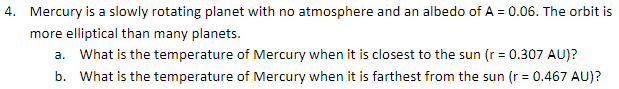
\includegraphics[scale = 0.8]{probset3num4.PNG}

Recall the formulas for the sub-solar temperature and power radiated temperature:
\begin{equation}
    T_P = 279(1-A)^{1/4}(\frac{r_p}{1 \:AU})^{-1/2}
\end{equation}
\begin{equation}
    T_{SS} = 395(1-A)^{1/4}(\frac{r_p}{1 \:AU})^{-1/2}
\end{equation}
I will inspect both of these temperatures.

a) We are given that the distance between the Sun and Mercury is $r_p = 0.307 \: AU$ and that the albedo of Mercury is $A = 0.06$. Plugging this into equation (4.1) we find that the power radiated temperature is
\[T_P = 279(1-0.06)^{1/4}(\frac{0.307 \: \cancel{AU}}{1 \: \cancel{AU}})^{-1/2}\]
\[ = 279(0.94)^{1/4}(0.307)^{-1/2}\]
\[\approx 495.8 \: K\]
Now to find the sub-solar temperature, plug in the value of $A$ and $r_p$ into equation (4.2), we find
\[T_{SS} = 395(1-0.06)^{1/4}(\frac{0.307 \: \cancel{AU}}{1 \: \cancel{AU}})^{-1/2}\]
\[ = 395(0.94)^{1/4}(0.307)^{-1/2}\]
\[ \approx 701.96 \: K\]
At Mercury's closest point to the Sun, we predict its temperature to lie in the range of $496 - 702 \:K$

b) Now let's find the power radiated and sub-solar temperatures when Mercury is at its furthest point from the sun ($r_p = 0.467 \: AU$). 
\[T_P = 279(0.94)^{1/4}(0.467)^{-1/2}\]
\[ \approx 402 \: K\]
Now the sub-solar temperature:
\[T_{SS} = 395(0.94)^{1/4}(0.467)^{-1/2}\]
\[\approx 569.14 \: K\]
At Mercury's furthest point, we predict that its temperature lies in the range of $ 402 - 569 \:K$.

\section{}
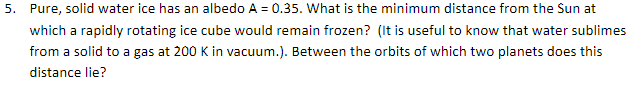
\includegraphics[scale = 0.8]{probset3num5.PNG}

We can expect that using the power radiated temperature will give the smallest value for the radius. I will find the radius when the power radiated temperature of solid water ice is equal to 200 $K$. 
\[T_{P} = 279(1-A)^{1/4}(\frac{r}{1 \:AU})^{-1/2} = 200 \:K\]
Solving for $r$, we find
\[r = (\frac{279}{200}(1-A)^{1/4}( 1 \:AU))^2\]
\[ = (\frac{279}{200}(0.65)^{1/4}(1 \:AU))^2\]
\[ \approx 1.57 \:AU\]
This outside a distance of approximately $1.57 \: AU$, we can expect that solid water ice will remain frozen. Notice that this distance lies between the orbits of Mars (1.5 AU) and Jupiter (5.2 AU).


\section{}
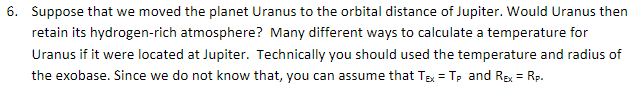
\includegraphics[scale = 0.8]{probset3num6.PNG}

Let's inspect the worst case scenario for Uranus at the distance of Jupiter. That is, assume that Uranus is a perfect blackbody, that is, $A = 0$ and use equation (4.2) to find the sub-solar temperature of Uranus at this distance:
\[T_{SS} = 395 \:K(\frac{r_{Uranus}}{1 \: AU})^{-1/2}\]
\[ = 395 \: K (5.2)^{-1/2}\]
\[ \approx 173.2 \:K\]
So our worst-case scenario temperature for Uranus is about 173.2 $K$. Now let's find the molecular mass of gasses that Uranus can retain. We will use the following formula:
\begin{equation}
    \mu \geq 7.1 (\frac{T_{Uranus}}{1000 \:K})(\frac{M_{Uranus}}{M_{Earth}})^{-1}(\frac{R_{Uranus}}{R_{Earth}})
\end{equation}
From the table at the top of the assignment, we can see that the mass and radius of Uranus are as follows:
\[M_{Uranus} = 14.5 \:M_{Earth}\]
\[R_{Uranus} = 3.98 \: R_{Earth}\]
Plugging these values into (6.1), we find
\[\mu \geq 7.1(\frac{173.2 \:\cancel{K}}{1000 \: \cancel{K}})(\frac{14.5 \:\cancel{M_{Earth}}}{\cancel{M_{Earth}}})^{-1}(\frac{3.98 \:\cancel{R_{Earth}}}{\cancel{R_{Earth}}})\]
\[ = 7.1(.1732)(\frac{1}{14.5})(3.98)\]
\[\approx 0.338\]
That is, Uranus can retain gasses with molecular masses of greater than 0.338. And since the molecular mass of hydrogen is 2, we can safely say that Uranus will retain its hydrogen-rich atmosphere if were located where Jupiter is.

\end{document}
